% Generated by pysimcount.pfboundratio -- do not edit; regenerate instead.
% figure: bound-ratio-suzuki4 -- Suzuki S4: Trotter number from each bound / measured r, against n
% metric=r_ratio gatebase=cz; geometric mean over seeds [1, 2, 3, 4, 5, 6, 7, 8, 9, 10], bars min-max; r_method=measured (denominator); bounds: Analytic bound, Minimised bound, Commutator bound (2018), Commutator bound (2021), Empirical fit (2018)
% sizes: np-main n = [4, 5, 6, 7, 8, 10]; np-main-n9 n = [9]; np-main-n11 n = [11]
% run set np-main-n9 made from uncommitted code (git_dirty), accepted: run at e42ff29 with the only modified tracked file pysimcount/pfseeds.py (an aggregation module the run does not import); checked with git diff --stat e42ff29 -- pysimcount/ on 2026-11-08
% run set np-main-n11 made from uncommitted code (git_dirty), accepted: run at e42ff29 with the only modified tracked file pysimcount/pfseeds.py (an aggregation module the run does not import); checked with git diff --stat e42ff29 -- pysimcount/ on 2026-11-08
% formulas: Suzuki S4
% figure made at git_commit=e5d9ee696f892e28aced765585653760f8a427c4 git_dirty=False
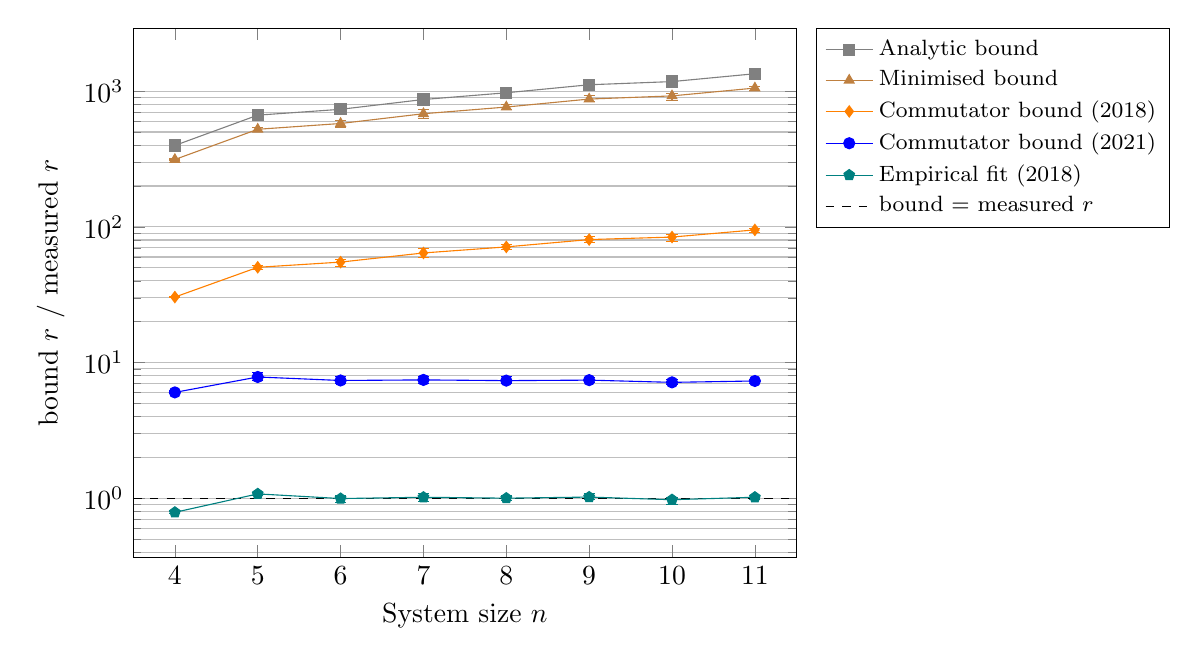
\begin{tikzpicture}
  \begin{semilogyaxis}[
    width=10cm, height=8.3cm,
    xlabel={System size $n$}, ylabel={bound $r$ / measured $r$},
    xmin=3.5, xmax=11.5,
    xtick={4,5,6,7,8,9,10,11},
    ymajorgrids=true, yminorgrids=true,
    legend pos=outer north east, legend cell align=left,
    legend style={font=\footnotesize},
  ]
    \addplot[dashed, black, domain=3.5:11.5, samples=2, forget plot] {1};
    \addplot[solid, gray, mark=square*, mark size=2pt, error bars/.cd, y dir=both, y explicit] coordinates {
      (4,397.817) -= (0,5.32805) += (0,3.59215)
      (5,665.095) -= (0,22.3246) += (0,20.5268)
      (6,734.402) -= (0,48.9232) += (0,38.1217)
      (7,867.205) -= (0,63.2616) += (0,62.0284)
      (8,972.123) -= (0,38.4125) += (0,37.0389)
      (9,1113.58) -= (0,49.1717) += (0,62.8709)
      (10,1175.29) -= (0,84.4823) += (0,45.1947)
      (11,1342.69) -= (0,54.9671) += (0,33.0138)
    };
    \addlegendentry{Analytic bound}
    \addplot[solid, brown, mark=triangle*, mark size=2pt, error bars/.cd, y dir=both, y explicit] coordinates {
      (4,313.397) -= (0,4.1974) += (0,2.82987)
      (5,523.337) -= (0,17.5663) += (0,16.1517)
      (6,577.363) -= (0,38.4619) += (0,29.9701)
      (7,681.295) -= (0,49.6996) += (0,48.7308)
      (8,763.292) -= (0,30.1607) += (0,29.0822)
      (9,873.956) -= (0,38.5909) += (0,49.3422)
      (10,922.027) -= (0,66.277) += (0,35.4555)
      (11,1053) -= (0,43.1077) += (0,25.891)
    };
    \addlegendentry{Minimised bound}
    \addplot[solid, orange, mark=diamond*, mark size=2pt, error bars/.cd, y dir=both, y explicit] coordinates {
      (4,30.3847) -= (0,0.406949) += (0,0.274364)
      (5,50.3354) -= (0,1.68956) += (0,1.5535)
      (6,54.987) -= (0,3.66304) += (0,2.85429)
      (7,64.2123) -= (0,4.68421) += (0,4.5929)
      (8,71.1672) -= (0,2.8121) += (0,2.71154)
      (9,80.582) -= (0,3.55823) += (0,4.54954)
      (10,84.0747) -= (0,6.04344) += (0,3.233)
      (11,94.9632) -= (0,3.88761) += (0,2.33494)
    };
    \addlegendentry{Commutator bound (2018)}
    \addplot[solid, blue, mark=oplus*, mark size=2pt, error bars/.cd, y dir=both, y explicit] coordinates {
      (4,6.03104) -= (0,0.144675) += (0,0.196234)
      (5,7.83347) -= (0,0.416803) += (0,0.655419)
      (6,7.38045) -= (0,0.366366) += (0,0.498337)
      (7,7.45372) -= (0,0.408775) += (0,0.433781)
      (8,7.36276) -= (0,0.287991) += (0,0.586738)
      (9,7.42535) -= (0,0.269609) += (0,0.383349)
      (10,7.14988) -= (0,0.231132) += (0,0.315396)
      (11,7.31942) -= (0,0.331044) += (0,0.192929)
    };
    \addlegendentry{Commutator bound (2021)}
    \addplot[solid, teal, mark=pentagon*, mark size=2pt, error bars/.cd, y dir=both, y explicit] coordinates {
      (4,0.788336) -= (0,0.0105584) += (0,0.00711841)
      (5,1.07785) -= (0,0.0361789) += (0,0.0332655)
      (6,0.995922) -= (0,0.0663448) += (0,0.0516968)
      (7,1.01809) -= (0,0.0742683) += (0,0.0728206)
      (8,1.00222) -= (0,0.0396017) += (0,0.0381855)
      (9,1.02129) -= (0,0.0450966) += (0,0.0576603)
      (10,0.976438) -= (0,0.0701881) += (0,0.0375479)
      (11,1.01844) -= (0,0.0416929) += (0,0.0250412)
    };
    \addlegendentry{Empirical fit (2018)}
    \addlegendimage{dashed, black}
    \addlegendentry{bound $=$ measured $r$}
  \end{semilogyaxis}
\end{tikzpicture}
